%---Titelseite------------------------------------------------------------------------------------


\documentclass{scrartcl}
\usepackage[utf8]{inputenc}
\usepackage[T1]{fontenc}
\usepackage[ngerman]{babel}
\usepackage{amsmath}
\usepackage{graphicx}

\newcommand{\HRule}{\rule{\linewidth}{0.5mm}}

\begin{document}


\begin{titlepage}
 
\begin{center}
 
 
% Upper part of the page
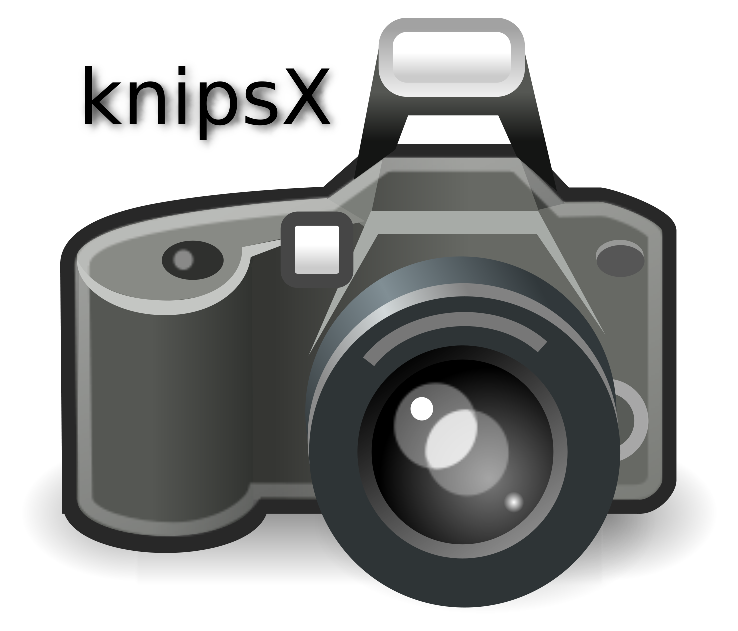
\includegraphics[width=0.33\textwidth]{cover.eps}\\[3cm]
 
\textsc{\LARGE Praxis der Softwareentwicklung}\\[1.5cm]
 
\textsc{\Large Gruppe 30}\\[0.5cm]
 
 
% Title
\HRule \\[0.4cm]
{ \huge \bfseries knipsX Entwurf}\\[0.4cm]
 
\HRule \\[1.5cm]
 
% Author and supervisor
\begin{minipage}{0.4\textwidth}
\begin{flushleft} \large

Gruppenmitglieder: \\
Borovik, Volodymyr \\
Bouché, Kai \\
Draxler, Benjamin \\
Kaufman, David \\
Zuber, Kevin

\end{flushleft}
\end{minipage}
\begin{minipage}{0.4\textwidth}
\begin{flushright} \large
Gruppenbetreuer: \\
Meder, David
\end{flushright}
\end{minipage} 
\vfill

% Bottom of the page
{\large \today ~- Revision: 1.0}
 
\end{center}
\end{titlepage}


Im folgenden Dokument sehen Sie den Entwurf von knipsX, spezifiert in UML 2.2. Auf den ersten Seiten befindet sich das Paketdiagramm, danach kommen die Klassendiagramme, die Sequenzdiagramme und noch eine Beschreibung aller Klassen mit deren Attributen und Methoden. Im Anhang finden sie noch eine Liste aller Klassen.

Den Diagrammen liegen folgende Legende zugrunde:
	Klassenfamilienfarben:
	\begin{enumerate}
		\item Rot: Externe Klassen meist Java SDK
		\item Grün: Alle Klassen die zur View gehören.
		\item Blau: Alle Klassen die, die zugrunde liegenden Daten bilden, sprich das Model.
		\item Gelb: Alle Klassen die für die Steuereung des Programms notwendig sind, sprich die Controller.
	\end{enumerate}
	Zudem befinden sich Kommentare in den Diagrammen, diese erkennt man an der umgeschlagenen Ecke und an der gelb-orangen Färbung.


\end{document}
